% !TEX root = ../main_v2.tex
\section{Numerical Validation}
\label{sec:numerical_results}

The exact solution of Sec.~\ref{sec:qubit_direct_response_v5} depends on the
bath only through the kernel evaluated at three frequencies,
$\omega \in \{0, \pm\omega_q\}$.
To test it we compare against Exact Diagonalisation (ED) of a truncated
spin-boson model: the qubit is coupled to $N_\omega$ harmonic oscillators,
each represented with a per-mode Fock cutoff $n_{\max}$.
A key feature of this comparison is that the analytic kernel integrals
$\mathcal{K}(\omega) = \int_0^\infty d\nu\, J(\nu)\, \mathcal{F}(\nu,\omega,\beta)$
can be evaluated in two ways: using the full continuum spectral density
(the \emph{continuous analytic} branch) or restricted to the same $N_\omega$
discrete modes seen by ED (the \emph{discrete analytic} branch).
These two branches have the same physical content but sample the spectral
density differently, and distinguishing between them is essential for
interpreting the comparison.

\subsection*{Discrete bath versus continuum: Fig.~\protect\ref{fig:ed_vs_analytic}}

Figure~\ref{fig:ed_vs_analytic} shows the excited-state population $p_{11}$
as a function of coupling strength (panel~a, $\beta\omega_q = 2$,
$\theta = \pi/4$) and inverse temperature (panel~b, $g/\omega_q = 0.5$,
$\theta = \pi/2$), each for $N_\omega = 40$ modes.
At weak coupling ($\chi \ll 1$) all three curves coincide: ED, the discrete
analytic, and the continuous analytic all agree to graphical precision.
As the system crosses into the strong-coupling regime ($\chi \gtrsim 1$,
past the vertical crossover markers $g_\star$ and $\beta_\star$), the
continuous analytic separates from ED while the discrete analytic continues
to track it closely.

The discrete analytic tracks ED by construction: both evaluate the kernel
on the same set of $N_\omega$ delta functions in the spectral density, so
their agreement is a self-consistency check rather than a physical
prediction.
The physically significant content is the \emph{divergence} of the
continuous analytic from ED, which grows with $\chi$.
This is not a failure of the theory.
The continuous analytic evaluates the kernel correctly in the thermodynamic
bath limit; as $\chi$ grows, its prediction departs from the $N_\omega$-mode
simulation because the finite discrete bath cannot reproduce the spectral
weight distribution of the continuum, in particular near the resonant
frequency $\omega_q$.
The correctness of the continuum formula is confirmed by its smooth
convergence to the ultrastrong limit $p_\infty$ (dashed lines), which
the finite ED bath cannot reach with any finite $N_\omega$.
The discrete analytic, using the same mode set as ED, follows the simulation
all the way to large $\chi$ and in doing so shows that the mismatch is
entirely due to bath discretisation, not to any deficiency in the formula.

\begin{figure}[t]
  \centering
  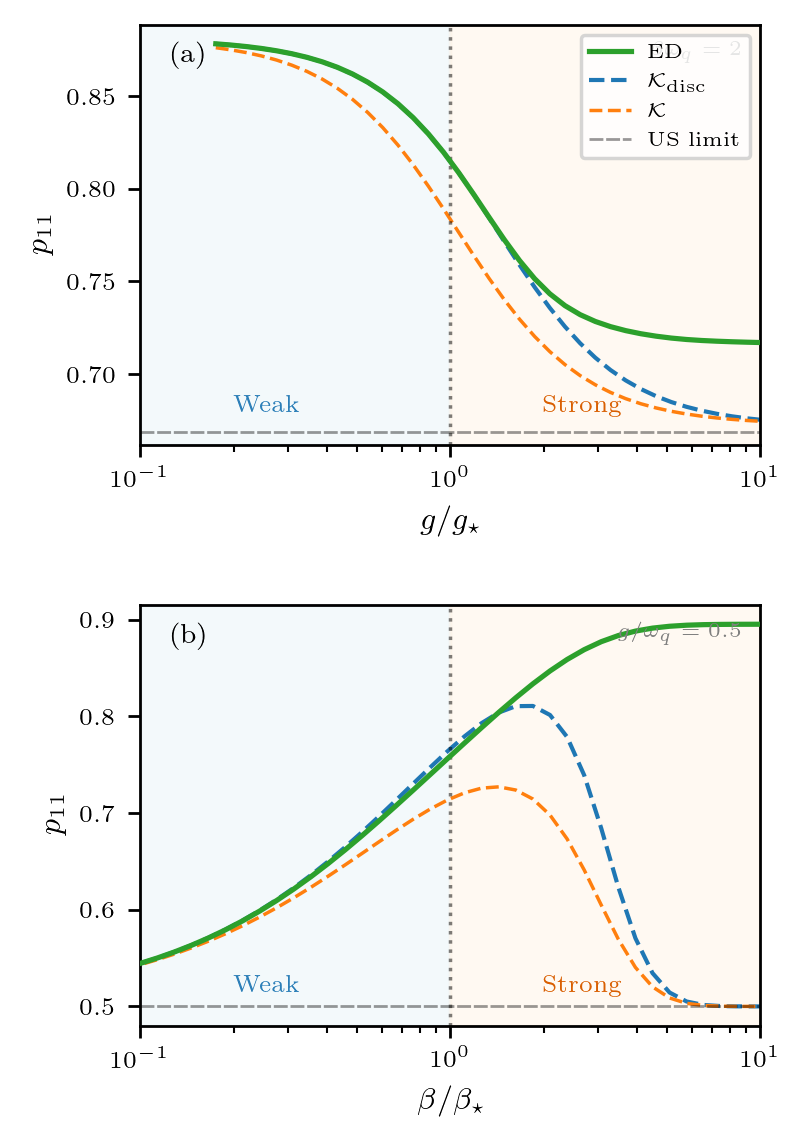
\includegraphics[width=0.48\textwidth]{../figures/hmf_fig2_ed_vs_analytic.png}
  \caption{Excited-state population $p_{11}$ along the coupling sweep
    (panel~a, $\beta\omega_q=2$) and the temperature sweep
    (panel~b, $g/\omega_q=0.5$) for $N_\omega=40$ modes.
    Green solid: ED.  Blue dashed: discrete analytic (same $N_\omega$ modes).
    Orange dotted: continuous analytic.
    Vertical dotted lines mark the crossover scales $g_\star$ and
    $\beta_\star$ calculated from $\chi(\beta,g)=1$.
    Dashed horizontal lines mark the ultrastrong limit $p_\infty$.
    The discrete analytic tracks ED throughout; the gap that opens between
    the continuous analytic and ED for $\chi\gtrsim1$ is a finite-bath
    discretisation artifact.}
  \label{fig:ed_vs_analytic}
\end{figure}

\subsection*{Spectral window and simulability: Fig.~\protect\ref{fig:bandwidth_convergence}}

The divergence of ED from the continuum prediction depends not only on
the number of modes $N_\omega$ but also on how those modes are distributed
across the spectral window $[\omega_{\min}, \omega_{\max}]$.
Figure~\ref{fig:bandwidth_convergence} examines this through a three-mode
bath ($N_\omega = 3$, $\omega_q = 2$, $g = 0.5$) with bandwidth
$B = \omega_{\max} - \omega_{\min}$ varied continuously.

Panel~(a) reveals a non-monotone RMSE: the error has a distinct minimum
near $B_{\mathrm{opt}} \approx 3.2$, rises sharply beyond the predicted
magic bandwidth $B^* = 2(\omega_q - \omega_{\min}) = 3.8$, and separates
strongly across Fock cutoffs $n_{\max} \in \{4,5,6\}$ only once $B > B^*$.
The physical origin of $B^*$ is that modes entering the spectral window
above $B^*$ are off-resonant from $\omega_q$ and, at any non-zero coupling,
acquire a large displacement in the dressed ground state; representing
these displaced oscillators faithfully requires higher Fock levels.
Panel~(b) shows that the resulting cutoff sensitivity $|p_{00}(n_{\max}=4)
- p_{00}(n_{\max}=6)|$ peaks sharply in $B \in [B_{\mathrm{opt}}, B^*]$
and is most pronounced at low temperature, consistent with the $\chi$
picture: a lower temperature raises $\chi$, tightening the resonance and
making the representation of off-resonant modes progressively more costly.
Panel~(c) confirms this directly: at fixed $B = B_{\mathrm{opt}}$, the
residual $|\Delta p_{00}|$ between ED and the ordered analytic grows
monotonically with $\beta$, with the curves for different $n_{\max}$
splitting at the same $\beta\omega_q \approx 2$ where $\chi \sim 1$.

\begin{figure*}[t]
  \centering
  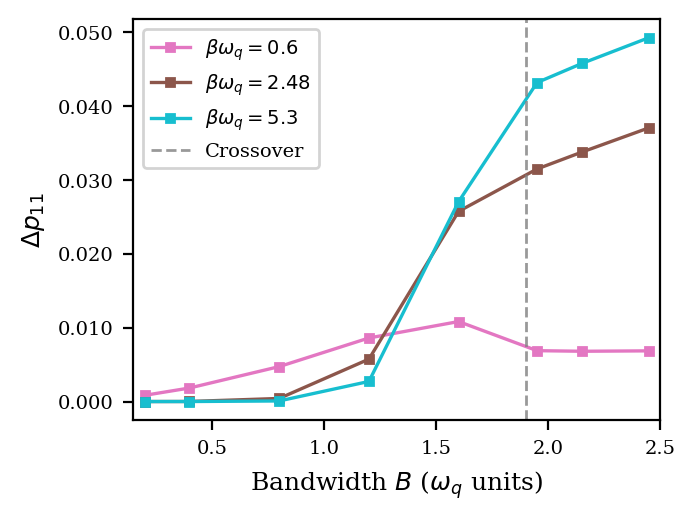
\includegraphics[width=0.95\textwidth]{../figures/hmf_fig3_bandwidth_convergence.png}
  \caption{ED simulability crossover as a function of spectral window
    bandwidth $B = \omega_{\max} - \omega_{\min}$.
    Parameters: $\omega_q = 2$, $g = 0.5$, $N_\omega = 3$;
    light-to-dark blue corresponds to $n_{\max} \in \{4,5,6\}$.
    \textit{Panel~(a)}: RMSE of $p_{00}$ versus bandwidth, averaged over
    inverse-temperature values $\beta\omega_q \in [0.6,10]$.
    The red dashed line marks the magic bandwidth $B^* = 3.8$; the green
    dash-dotted line marks the empirical RMSE minimum $B_{\mathrm{opt}} = 3.2$.
    \textit{Panel~(b)}: Cutoff sensitivity $|p_{00}(n_{\max}=4) -
    p_{00}(n_{\max}=6)|$ versus bandwidth at three representative
    temperatures; sensitivity is largest at low temperature ($\chi$ largest).
    \textit{Panel~(c)}: Absolute residual $|\Delta p_{00}|$ versus
    temperature at fixed $B = B_{\mathrm{opt}}$; curves for all three
    cutoffs split below $\beta\omega_q \approx 2$ where $\chi$ crosses unity.}
  \label{fig:bandwidth_convergence}
\end{figure*}

Together, Figs.~\ref{fig:ed_vs_analytic} and~\ref{fig:bandwidth_convergence}
establish that the analytic result is correct and parameter-free: where ED
agrees, it does so because the discrete and continuous kernels coincide, and
where they differ, the exact formula identifies the discretisation artifact
via the crossover scale $\chi$.
The simulability of the finite bath is itself a physical quantity,
transparently controlled by the same parameter that governs the
weak-to-ultrastrong crossover of the reduced state.
